\chapter{Implementation}
In this chapter, we will present implementation details of our system. First, we present all libraries used in this project. Later we will introduce outcome in the form of the \gls{ROS} package. Also, we will briefly present the structure of the program and key components.
\section{Used libraries}
\subsection {\gls{ROS}}
The \gls{ROS} \cite{ros_papper} is a popular robotic framework. It offers a flexible way how to combine existing tools, libraries, and algorithms to make a full robotic solution from drivers up to the higher logic of planning and mapping. The communication between individual programs (nodes) is done through the subscriber-publisher model. A configuration of programs is stored in the parameter server. This server also takes care of managing communication between nodes. 
\subsection{The Point Cloud library}
The \gls{PCL} is a standard \gls{ROS} library for manipulation with point clouds \cite{pcl}. The library includes state-of-the-art algorithms in registration, filtering, segmentation, and feature extraction. It also contains tools for visualization and manipulation with point clouds. In our project, we use mostly point cloud class which is the most basic data structure in the library. We also use registration base class for implementation of our scan matching algorithms. 
\subsection{The G2O}
The G2O is a pose graph optimization library presented by \cite{g2o}. It is currently the most used library for the pose graph optimization. It offers well designed extendable interface which makes it easy to add a new definition of pose graph optimization. New optimization methods often have an implementation for this library. In our program, it is used as main optimization engine for our pose graph.
\subsection{The Eigen}
The Eigen \cite{eigenweb} is a templated C++ library for linear algebra. It includes modules for dense and sparse matrix representations, numerical solvers and transformation representation. This project mostly uses geometry module with affine transformation. We also utilize numerical solvers in our implementation of registration algorithms. We have selected this library because it is considered a standard library for linear algebra in the \gls{ROS}. Many packages use it and offer API's designed with this library.   

\section{Structure of the implementation}
 The architecture of the whole system can be divided into three parts. The first part is the\gls{ROS} interface. In our implementation, this interface expects only laser scanner data. However, it is also possible to provide odometry information.  The interface uses standard names for topics. This interface includes all inputs and outputs which can be found in other SLAM packages. Additionally, it provides a map in the form of a point cloud. The full documentation of this interface is in Appendix \ref{chap:ndt_gslam_package}.
 
 The second part is the SLAM algorithm interface implemented in C++. It offers the same functionality as the ROS interface. We have decided to have this double interface because it is convenient to use our SLAM also without the \gls{ROS} subscribe-publish interface. It was mainly used for debugging and testing purposes. This interface also offers some flexibility if we decide to do a different version of our algorithm. In this case, we do not have to rewrite node's source code. In this layer of abstraction, we take care of an initial estimation of the odometry and the \gls{NDT} frame building process. A map generation also takes place in this part of the architecture.
 
 Thirds part is graph \gls{SLAM} interface. This interface makes abstraction around graph creation and optimization process. This section is using our custom pose graph implementation. On top of this graph, we developed a loop closure detection and validation. This graph is synchronized with the graph inside of optimization engine G2O. We carry two graphs for the reason of easier switching between different optimization engines in the future. Our graph representation also includes additional information about state and type of the edge. Implementing it into G2O would require rewriting this code with every new optimizer and with every new G2O edge and vertex type.
 
 An important part of the architecture is handling of \gls{NDT} frames. A created frame is stored inside shared pointer. The same pattern is used in \gls{PCL}'s point cloud data type. The shared pointer is then passed to the graph creation process and also to the \gls{NDT} map building process. Nodes of the pose graph include this pointer as their representation of the world. The \gls{NDT} frames in nodes are used for loop closure registration. This means that registration algorithms use the shared pointers in their API as well. This approach is also a standard for registration algorithm in the \gls{PCL} library
 
 \begin{figure}
 	\centering
 	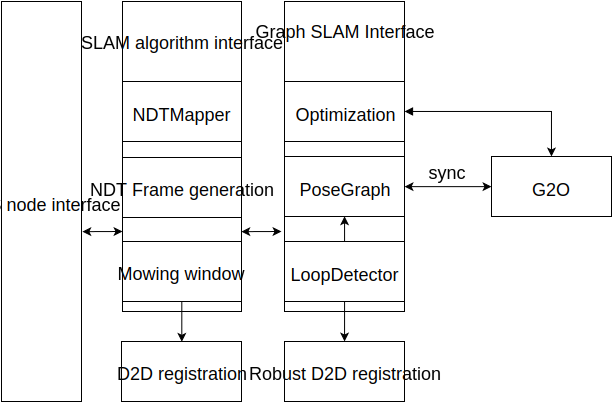
\includegraphics[width=140mm]{../img/architecture.png}
 	\caption{Overview of individual parts of architecture and their relationships.}\label{fig:architecture}
 \end{figure}
      
\subsection{NDTGrid2D}
The NDTGrid2D is the main class for all operations in our approach. It offers basic functionality for grid creation. It can be merged with or without a use of ray-tracing (occupancy update). It is used for dynamic entity update from \gls{NDT-OM}. It also offers grid translation which is needed for the moving window implementation. Another group of functionality is for registration algorithms. They require radius search and k-nearest neighbor search. The odometry estimator also needs to use means from cells. The last group is output format methods. Grid can create a coarser instance of itself. It is also able to be printed to standard console output. We have implemented methods for conversion into our custom type of occupancy and \gls{NDT} map messages. These messages are used only internally and can be transformed into \gls{ROS} variants.

In order to fulfill all these needs implementation of NDTGrid2D is just a higher abstraction layer on top of the VoxelGrid2D. The voxel grid is taking care of memory layout, resizing, element lookup and ray-tracing. The NDTGrid2D has two template parameters. The first parameter is the type of the cell. Grid is initialized from a point cloud, for this reason, it needs to have second template parameter representing a type of the point. The second parameter is standardly used in \gls{PCL} related algorithms.  

Core algorithm logic for merging and updating cells is stored in every cell. This allows developing new cells without any changes to the grid.
\subsection{VoxelGrid2D}
It is a generic grid-like structure with one template parameter. The type used in the template is required to have implemented operator plus and copy assignment. This data structure is intended to use with larger cell types in the sparse environment. Based on these requirements we designed the memorry model. Grid is represented by single vector which holds pointers to cells. In the case of the unoccupied cell, it uses null pointers. The grid is initialized empty with no cells inside. It allows dynamic resizing either manual or automatic based on inputted cells.  It offers base functionality for ray-tracing and radius search. 
\subsection{NDTCell}
The \gls{NDT} cell is the core of all calculations on top of the grid. In case of \gls{NDT-OM} implementation it holds covariance and mean estimation, occupancy update rule and \gls{RCU} update rule for merging of cells with Gaussian inside. In the future experiments we can easily design a new type of the cell with different calculation model and keep NDTGrid2D and the VoxelGrid without modifications.
\subsection{Registration algorithms}
When designing registration algorithms we have decided to use same interface as \gls{PCL}'s registration algorithms. By extension of their base class our programs can be used standard way inside of \gls{PCL}. This makes it easy to use our algorithms alongside \gls{PCL} implementations. It also possible to use all visualization and io tools provided by \gls{PCL}. Our algorithms have option to run in multiple threads which boost their performance on the multi-core processors. 

